\section{Statistical Analysis}
\label{sec:statistical_analysis}

\todo[inline]{Fit, limits, treatment of systematics in fit}

\subsection{Binning Algorithm}
\label{sec:binning_alg}


\subsection{Results}

\begin{figure}[htbp]
  \centering

  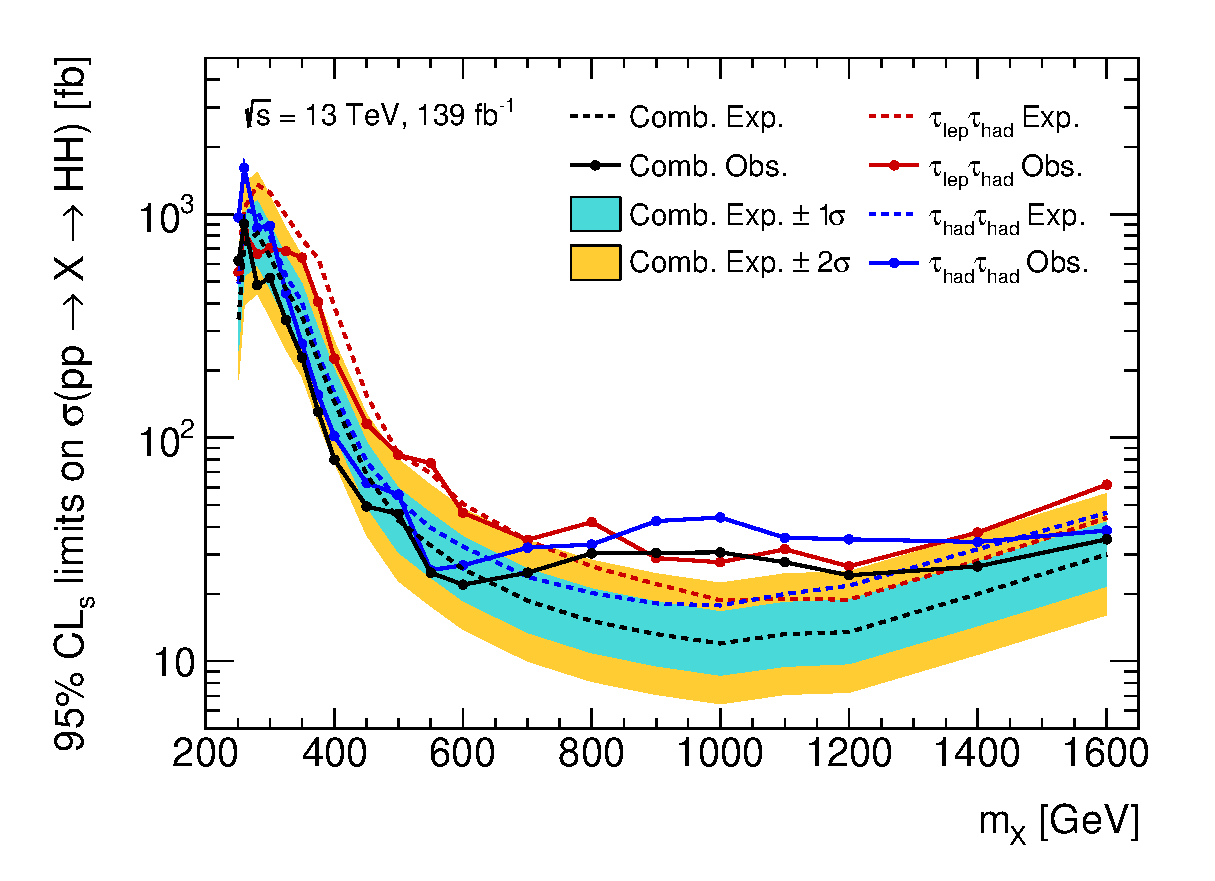
\includegraphics[width=0.65\textwidth]{results/resonant_comb_upper_limits}

  \caption{Upper limits for the resonant search}
  \label{fig:res_upper_limits}
\end{figure}

\begin{figure}[htbp]
  \centering

  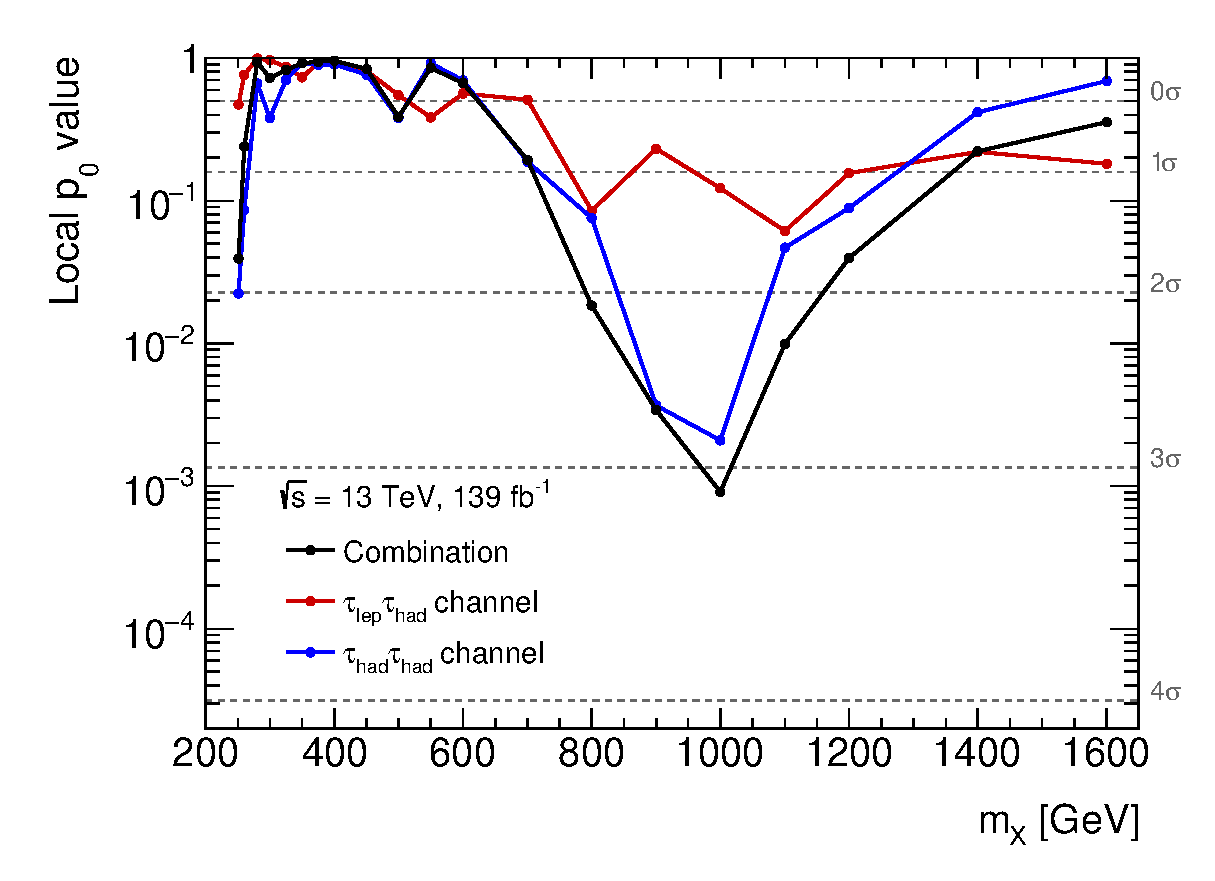
\includegraphics[width=0.65\textwidth]{results/resonant_comb_pvalues}

  \caption{Local pvalue scan}
  \label{fig:local_pvalues}
\end{figure}

\subsection{Discussion}



\begin{table}[htbp]
  \centering

  \begin{tabular}{lSS}
    \toprule
    & \multicolumn{2}{c}{Expected number of events} \\
    Process & {Last two bins} & {Last bin} \\
    \midrule
    \ZHF & 6.9 & \\
    Single Higgs boson & 6.9 & \\
    \ttbar & 4.6 & \\
    \jettotauhadvis (\ttbar) & 3.4 & \\
    \jettotauhadvis (multi-jet) & 2.2 & \\
    Other & 1.8 & \\
    \midrule
    Total background & & \\
    \midrule
    SM \HH (gluon fusion) & & \\
    SM \HH (VBF) & & \\
    \bottomrule
  \end{tabular}

  \caption{Table of expected yields. The uncertainties are from
    statistical sources only.}
  \todo[inline]{Post-fit yields}
\end{table}


%%% Local Variables:
%%% mode: latex
%%% TeX-master: "../../phd_thesis"
%%% End:
